\documentclass{beamer}

\mode<presentation> {


\usetheme{default}
% \setbeamertemplate{footline} % To remove the footer line in all slides uncomment this line
\setbeamertemplate{footline}[page number] % To replace the footer line in all slides with a simple slide count uncomment this line
\setbeamertemplate{navigation symbols}{} % To remove the navigation symbols from the bottom of all slides uncomment this line
}

\usepackage{graphicx} % Allows including images
\usepackage{booktabs} % Allows the use of \toprule, \midrule and \bottomrule in tables
\usepackage{verbatim}
\usepackage{multicol}

\title[VE215 RC1]{VE215 RC1}
\author{Erdao Liang, Chongye Yang}
\institute[UM-SJTU JI] 
{UM-SJTU JI}
\date{\today}

\begin{document}

\AtBeginSection[ ]
{
\begin{frame}{Overview}
    \tableofcontents[sectionstyle=show/shaded,subsectionstyle=show/shaded/hide]
 \end{frame}
}

%%%%%%%%%%%%%%%%%%%%%%%%%%%%%%%%%%%%%%%%%%%%%%%%%%%
% TITLE PAGE
\begin{frame}
\titlepage % Print the title page as the first slide
\end{frame}

%%%%%%%%%%%%%%%%%%%%%%%%%%%%%%%%%%%%%%%%%%%%%%%%%%%
% OVERVIEW
% \begin{frame}
% \frametitle{Overview}
% \tableofcontents
% \end{frame}

%%%%%%%%%%%%%%%%%%%%%%%%%%%%%%%%%%%%%%%%%%%%%%%%%%%
% LOGISTICS
\section{General Infomation}

%%%%%%%%%%%%%%%%%%%%%%%%%%%%%
\begin{frame}{Logistics}
    \begin{itemize}
        \item Office hour time

        Erdao Liang's OH: Wed. 20:30-22:30, LBL 326D.
        
        Chongye Yang's OH: Thu. 20:30-20:30, LBL 326C.

        
        \item Lab time
        
        Fri. 18:20-20:30, starting from Week 3.

        Do read the lab manual in advance!
        
    \end{itemize}
\end{frame}

%%%%%%%%%%%%%%%%%%%%%%%%%%%%%
\begin{frame}{Course Structure}
    \begin{itemize}
        \item Goal: analyze the circuits, from simple to complex.
        \item Structure:

        \begin{enumerate}
            \item Chap. 1-8: DC circuits (the circuits driven by constant current/voltage sources)

            A variety of analysis tools 
            
            $\rightarrow$ introducing some new circuits components 
            
            $\rightarrow$ analyze circuits with those complex components added
            
            \item Chap. 9-14: AC circuits (the circuits driven by alternating current/voltage sources)
        \end{enumerate}
        

    \end{itemize}
    
\end{frame}


%%%%%%%%%%%%%%%%%%%%%%%%%%%%%%%%%%%%%%%%%%%%%%%%%%%
% BASIC CONCEPTS
\section{Basic Concepts}

%%%%%%%%%%%%%%%%%%%%%%%%%%%%%
\begin{frame}{Current}

$$i \overset{\Delta}{=} \dfrac{\mathrm{d}q}{\mathrm{d}t}$$
$$Q \overset{\Delta}{=} \int_{t_{0}}^{t}i \mathrm{d}t $$

\textbf{Reference direction of current}

In solving problems, it does not matter which direction we initially assume. If we obtain a result of negative current, it indicates that the actual direction is opposite to that we have initially assumed.

\begin{figure}
\centering
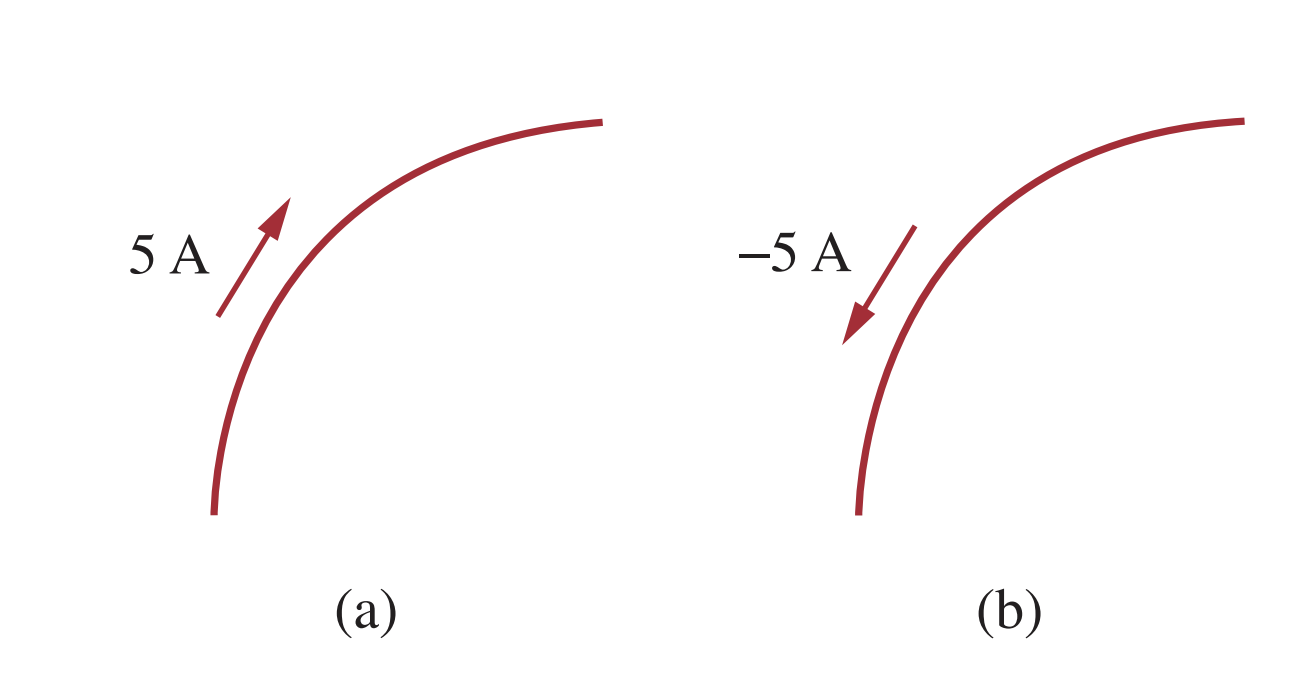
\includegraphics[width=0.6\textwidth]{current2.png}
\end{figure}

\end{frame}

%%%%%%%%%%%%%%%%%%%%%%%%%%%%%
\begin{frame}{Voltage}

$$ v_{ab} = v_a - v_b$$
$$ v_{ab} \overset{\Delta}{=} \dfrac{\mathrm{d}w}{\mathrm{d}q}$$

\textbf{Reference direction of voltage}

In solving problems, it does not matter how we assign the ``+/-" signs to two terminals of a circuit element. The two representations below are equivalent.



\begin{figure}
\centering
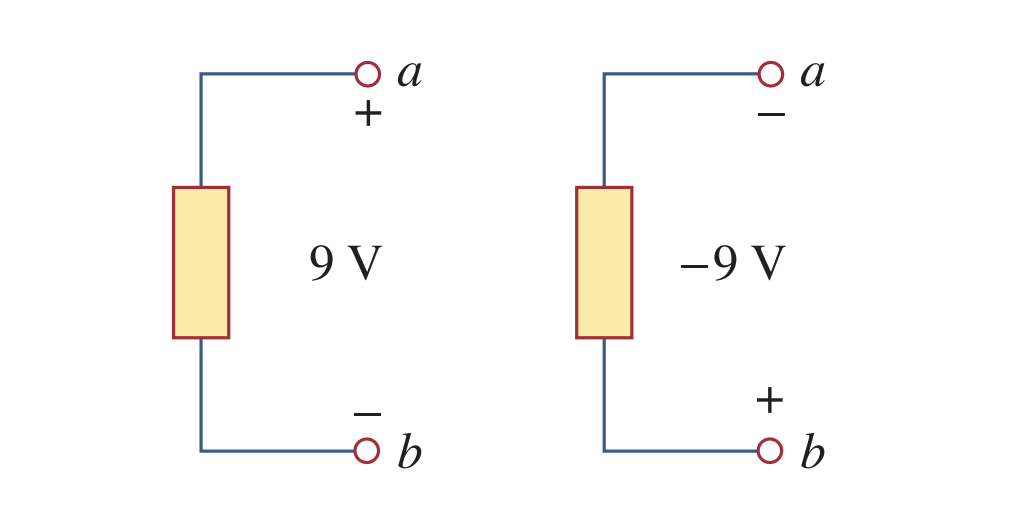
\includegraphics[width=0.6\textwidth]{voltage2.png}
\end{figure}
\end{frame}


%%%%%%%%%%%%%%%%%%%%%%%%%%%%%
\begin{frame}{Power and Energy}

$$p = \dfrac{\mathrm{d}w}{\mathrm{d}t} = vi \qquad w = \int_{t_0}^{t}vidt$$
Passive sign convention w.r.t. power:
\begin{itemize}
    \item Currents enter through the positive terminal: $p=+vi$
    \item Currents enter through the negative terminal: $p=-vi$

    \begin{figure}
    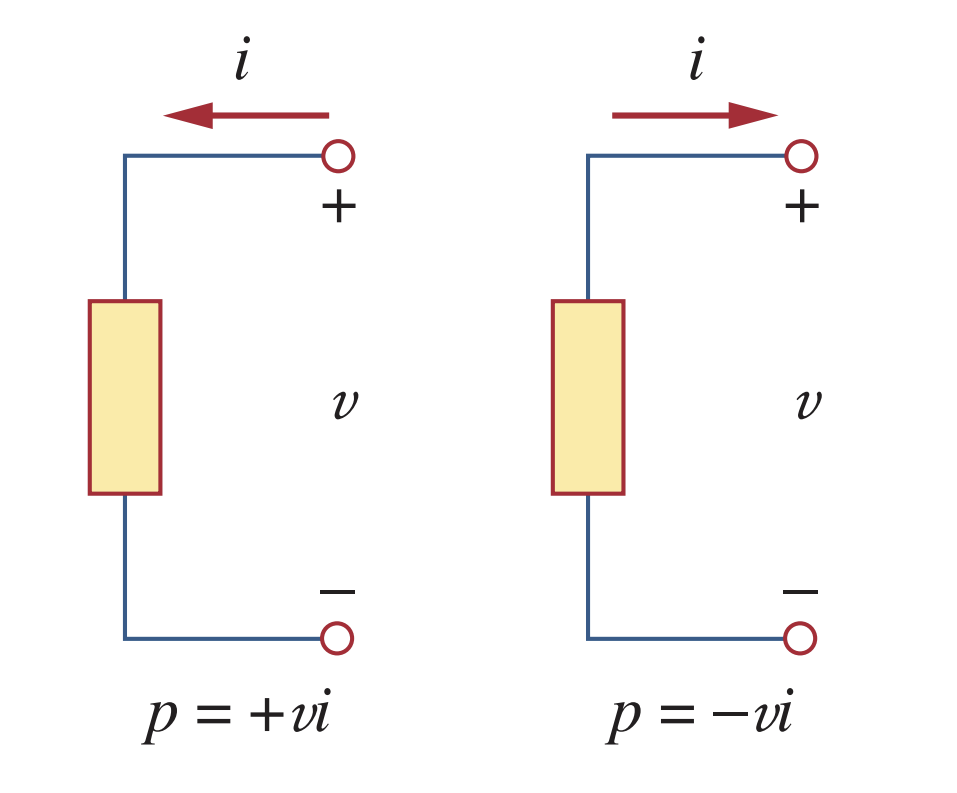
\includegraphics[width=0.3\textwidth]{power sign.png}
    \end{figure}
\end{itemize}
Power and energy consumption:
\begin{itemize}
    \item $p>0$, element consumes energy.
    \item $p<0$, element generates energy.
\end{itemize}

\end{frame}


%%%%%%%%%%%%%%%%%%%%%%%%%%%%%
\begin{frame}{Circuit Elements}

\begin{itemize}
\item \textbf{Active elements}: can generate energy

e.g., generators, batteries, operational amplifiers

\begin{itemize}
\item \textbf{independent source}: the source whose quantity is uninfluenced by its ``surroundings".
\begin{figure}
\flushleft
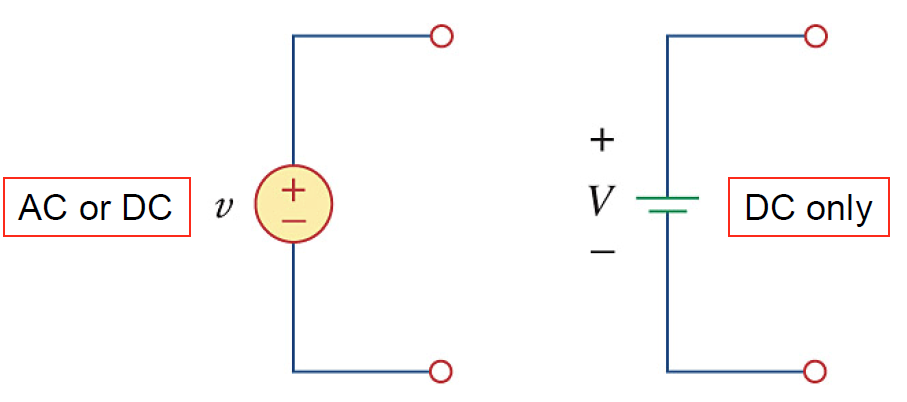
\includegraphics[width=1.5in]{12.png}
\end{figure}
\item \textbf{dependent source}: source quantity is controlled by another voltage or current in the circuit.
\begin{figure}
\flushleft
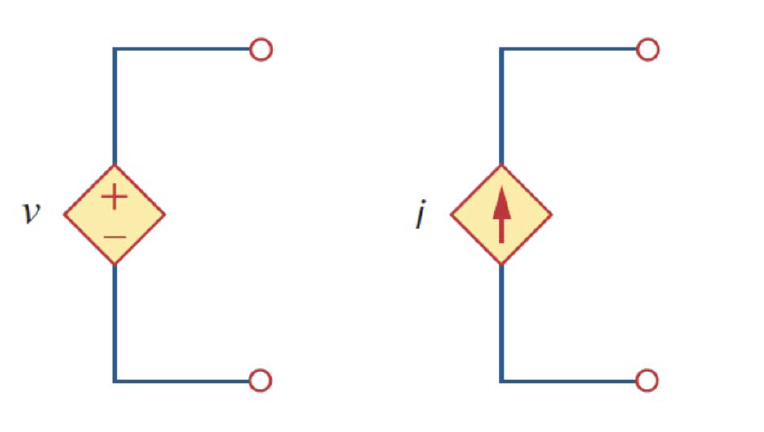
\includegraphics[width=1.4in]{13.png}
\end{figure}
\end{itemize}
\item \textbf{Passive elements}: cannot generate energy,
\newline
e.g., resistors, capacitors, inductors
\newline
\end{itemize}
\end{frame}

%%%%%%%%%%%%%%%%%%%%%%%%%%%%%%%%%%%%%%%%%%%%%%%%%%%
% BASIC LAWS
\section{Basic Laws}

%%%%%%%%%%%%%%%%%%%%%%%%%%%%%
\begin{frame}{Nodes, Meshes and Loops}
\textbf{Branch:} a single element, such as a voltage source or a resistor

\textbf{Node:} the point of connection between two or more branches

\textbf{Loop:} any closed path in a circuit
\begin{itemize}
\item \textbf{Mesh:} a loop that does not enclose any other 
loops, i.e., smallest loop
\item \textbf{Independent loop:} a loop that contains at least one branch which is not a part of any other independent loop
\end{itemize}


Fundamental theorem of network topology:
$$b\text{ (branches)}=l\text{(mesh)}+n\text{ (nodes)}-1$$
\end{frame}

%%%%%%%%%%%%%%%%%%%%%%%%%%%%%
\begin{frame}{Exercise}
\begin{enumerate}
\item Suppose there are 3 meshes and 6 branches in one circuit. 
\newline
How many nodes in it?
\newline
\item Count the number of nodes, branches, meshes, loops in the following figure.
\end{enumerate}
\begin{figure}
\centering
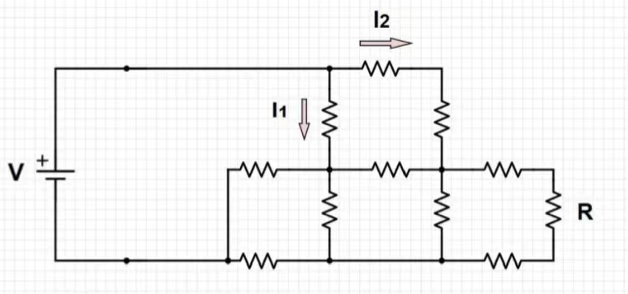
\includegraphics[width=2.5in]{q2.jpg}
\end{figure}
\end{frame}

%%%%%%%%%%%%%%%%%%%%%%%%%%%%%
\begin{frame}{Exercise}
\begin{enumerate}
\item Suppose there are 3 meshes and 6 branches in one circuit. 
\newline
How many nodes in it?
\\
\textbf{Answer:} 4
\item Count the number of nodes, branches, meshes, loops in the following figure.
\\
\textbf{Answer:} 8,12,5,21
\end{enumerate}
\begin{figure}
\centering
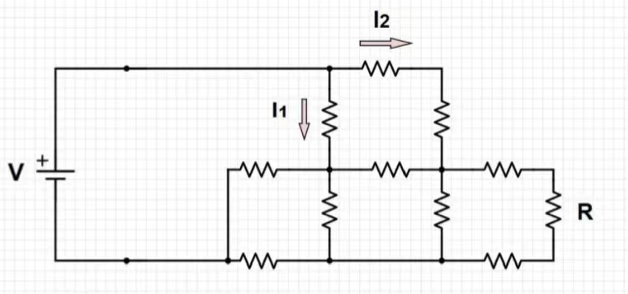
\includegraphics[width=2.5in]{q2.jpg}
\end{figure}
\end{frame}

%%%%%%%%%%%%%%%%%%%%%%%%%%%%%
\begin{frame}{Ohm's Law}


\begin{figure}
\centering
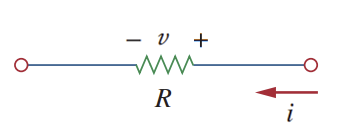
\includegraphics[width=0.4\textwidth]{ohm.png}
\end{figure}

Ohm's law:
$$V=IR \qquad R = \frac{v}{i}$$

Passive sign convention for Ohms's law:
\begin{itemize}
    \item $i$ enters through the positive terminal: $v=iR$
    \item $i$ enters through the negative terminal: $v=-iR$
\end{itemize}


\textbf{Not all resistors obey Ohm's law!}

A resistor that obeys Ohm's law is known as \textbf{a linear resistor}, i.e., a constant resistance.

\end{frame}

%%%%%%%%%%%%%%%%%%%%%%%%%%%%%
\begin{frame}{Resistance with extreme values}
\begin{enumerate}
    \item Short circuit: a circuit element with resistance approaching zero.
    \item Open circuit: a circuit element with resistance approaching infinity.
\end{enumerate}
\begin{figure}
\centering
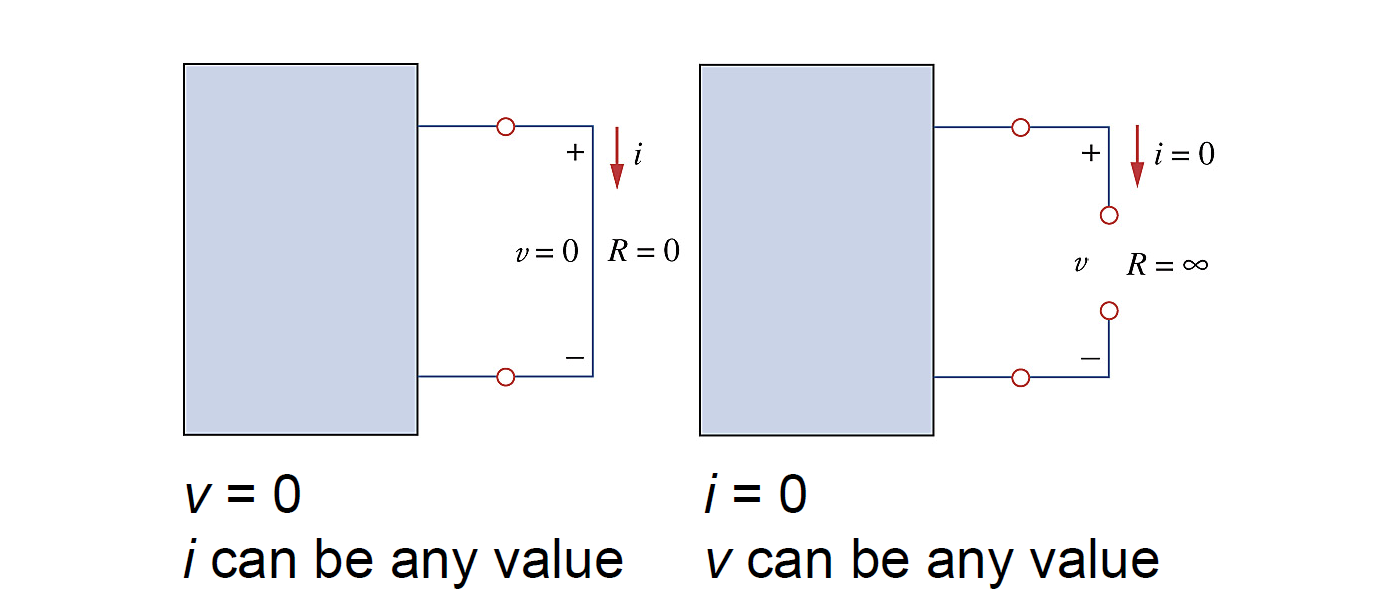
\includegraphics[width=0.8\textwidth]{16.png}
\end{figure}
\end{frame}

%%%%%%%%%%%%%%%%%%%%%%%%%%%%%
\begin{frame}{Conductance}
\begin{equation*}
G=\dfrac{1}{R}=\dfrac{i}{v},\ 
1S=1\mho=1A/V
\end{equation*}
where \textbf{G} is the conductance, \textbf{S} (siemens) is the SI unit of conductance and $\mho$ is the reciprocal ohm.
\par
some useful formula:
$$i=Gv,p=vi=i^{2}R=\dfrac{v^2}{R}=v^{2}G=\dfrac{i^{2}}{G}$$
\end{frame}

%%%%%%%%%%%%%%%%%%%%%%%%%%%%%
\begin{frame}{Kirchhoff's Law}
\begin{table}[]
    \centering
    \begin{tabular}{ccc}
        \toprule
        Kirchhoff's Law & Expression & Based on \\
        \midrule
        KCL & $\sum i_k = 0$ for a node & Conservation of charge\\
        KVL & $\sum v_k = 0$ for a mesh & Conservation of energy\\
        \bottomrule
    \end{tabular}
\end{table}


\begin{multicols}{2}
    \sectiont{}
    \begin{figure}
    \centering
    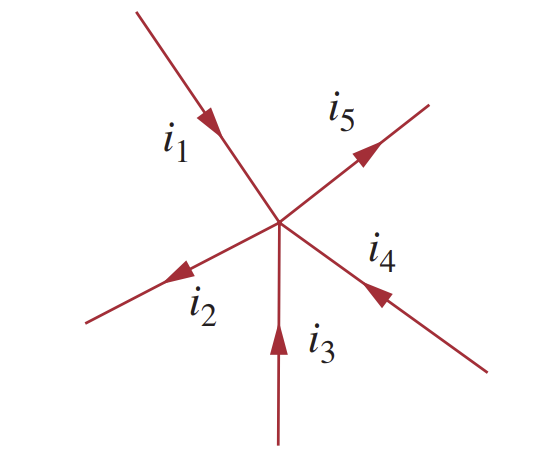
\includegraphics[width=0.33\textwidth]{24.png}
    \caption{KCL}
    \end{figure}
    \sectiont{}
    \begin{figure}
        \centering
        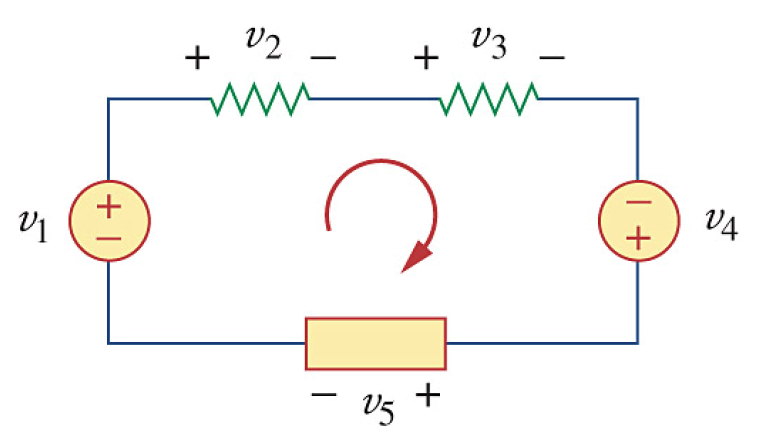
\includegraphics[width=0.48\textwidth]{25.png}
        \caption{KVL}
    \end{figure}
    
    
\end{multicols}
\end{frame}

%%%%%%%%%%%%%%%%%%%%%%%%%%%%%
\begin{frame}{KCL}
\textbf{KCL:} the algebraic sum of currents entering \textbf{a node (or a closed boundary)} is zero.

Steps of applying KCL:
\begin{enumerate}
    \item Find out all branches connected to the node of interest.
    \item Specify \textbf{reference} direction for current on each branch.
    \item Find all $i_k (k=1,2,\cdots,n)$ (Ohm's law $i=\frac{v_a-v_b}{R}$ for linear resistors).
    \item List the KCL equation $\sum_{k} i_k = 0$.
\end{enumerate}



\end{frame}

%%%%%%%%%%%%%%%%%%%%%%%%%%%%%
\begin{frame}{KVL}
\textbf{KVL:} the algebraic sum of all voltages around \textbf{a closed path (or loop)} is zero.

Steps of applying KVL:
\begin{enumerate}
    \item Select reference KVL direction (clockwise by convention).
    \item Confirm/specify the +/- terminal of each branch.
    \item Find $v_k (k=1,2,\cdots,n)$ for each branch.
    \item List the KVL equation $\sum_kv_k=0$. Mind that by passive sign convention, the sign in front of a certain term $v_k$ is 
    \begin{itemize}
        \item ``+" if the reference KVL direction enters through the positive terminal of the branch.
        \item ``-" if the reference KVL direction enters through the negative terminal of the branch.
    \end{itemize}
\end{enumerate}

\end{frame}

%%%%%%%%%%%%%%%%%%%%%%%%%%%%%
% \begin{frame}{Exercise}


% In the circuit below, determine $v_x$ and the power absorbed by the $12-\Omega$ resistor.
% \begin{figure}[H]
% \centering
% 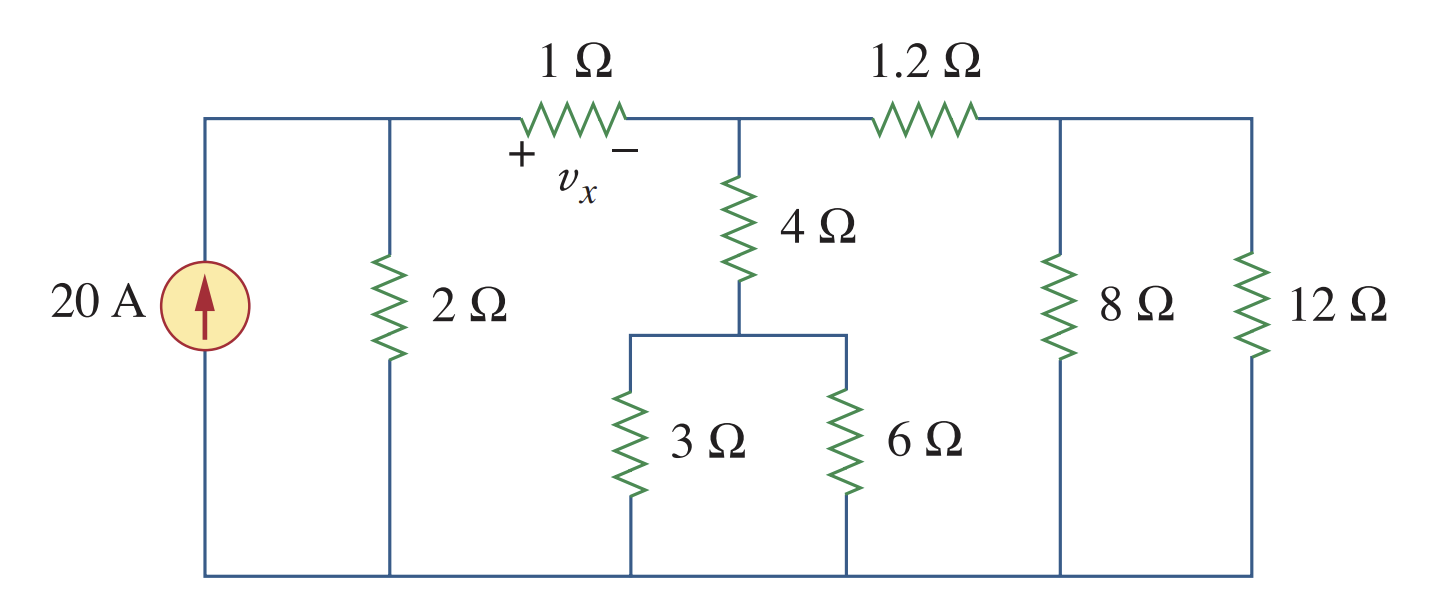
\includegraphics[width=0.8\textwidth]{KVLexercise.png}
% \end{figure}

% \begin{tiny}
% Steps of applying KVL:
% \begin{enumerate}
%     \item Select reference KVL direction (clockwise by convention).
%     \item Confirm/specify the +/- terminal of each branch.
%     \item Find $v_k (k=1,2,\cdots,n)$ for each branch.
%     \item List the KVL equation $\sum_kv_k=0$. Mind that by passive sign convention, the sign in front of a certain term $v_k$ is
     
%      ``+" if the reference KVL direction enters through the positive terminal of the branch.
     
%     ``-" if the reference KVL direction enters through the negative terminal of the branch.
    
% \end{enumerate}
% \end{tiny}

% \end{frame}

% %%%%%%%%%%%%%%%%%%%%%%%%%%%%%
% \begin{frame}{Exercise}


% \end{frame}


%%%%%%%%%%%%%%%%%%%%%%%%%%%%%
\begin{frame}{Series connection and Parallel connection}
$R_{eq}$: the \textbf{equivalent resistance}


\begin{enumerate}
    \item \textbf{Series} connection:
    $$R_{eq}=R_1+R_2+…+R_N=\sum_{n=1}^{N}R_{n}$$

    Principle of voltage division: $v_n = \frac{R_n}{\sum_{n=1}^{N} R_n}v$
    
    \item \textbf{Parallel} connection:
    $$G_{eq}=\frac{1}{R_{eq}} = G_1+G_2+…+G_N=\sum_{n=1}^{N}G_{n}$$

    Principle of voltage division: $i_n = \frac{G_n}{\sum_{n=1}^{N} G_n}i$
\end{enumerate}


\end{frame}

%%%%%%%%%%%%%%%%%%%%%%%%%%%%%
\begin{frame}{Wye-Delta Transformation}

\begin{itemize}
    \item Motivation: simplify the circuits for easier calculation.

    \item Two forms of special circuit connections:
    \begin{multicols}
        \sectiont{}
            \begin{figure}[H]
            \centering
            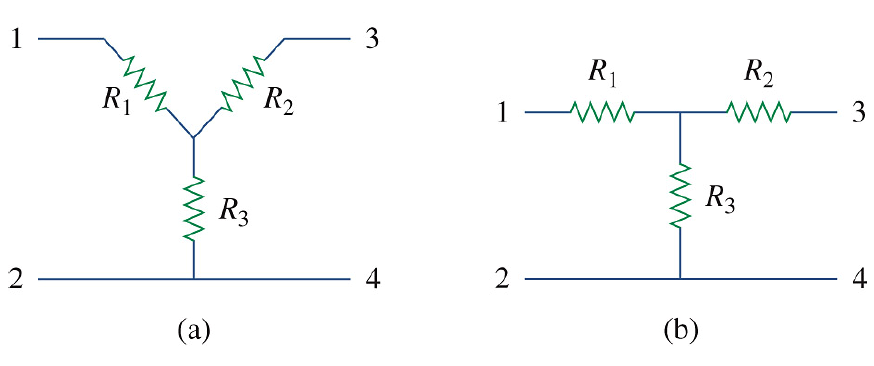
\includegraphics[width=0.45\textwidth]{Y.png}
            \caption{Wye (Y or T)}
            \end{figure}
        \sectiont{}
            \begin{figure}[H]
            \centering
            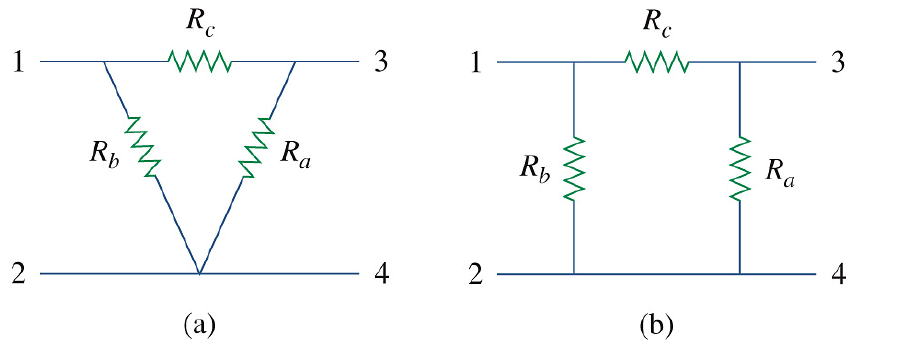
\includegraphics[width=0.5\textwidth]{DELTA.png}
            \caption{Delta ($\Delta$ or $\pi$)}
            \end{figure}
        
    \end{multicols}
    \item Goal: transform one type of connection into another.
\end{itemize}

\end{frame}

%%%%%%%%%%%%%%%%%%%%%%%%%%%%%
\begin{frame}{Wye-Delta Transformation}
\begin{figure}[H]
\centering
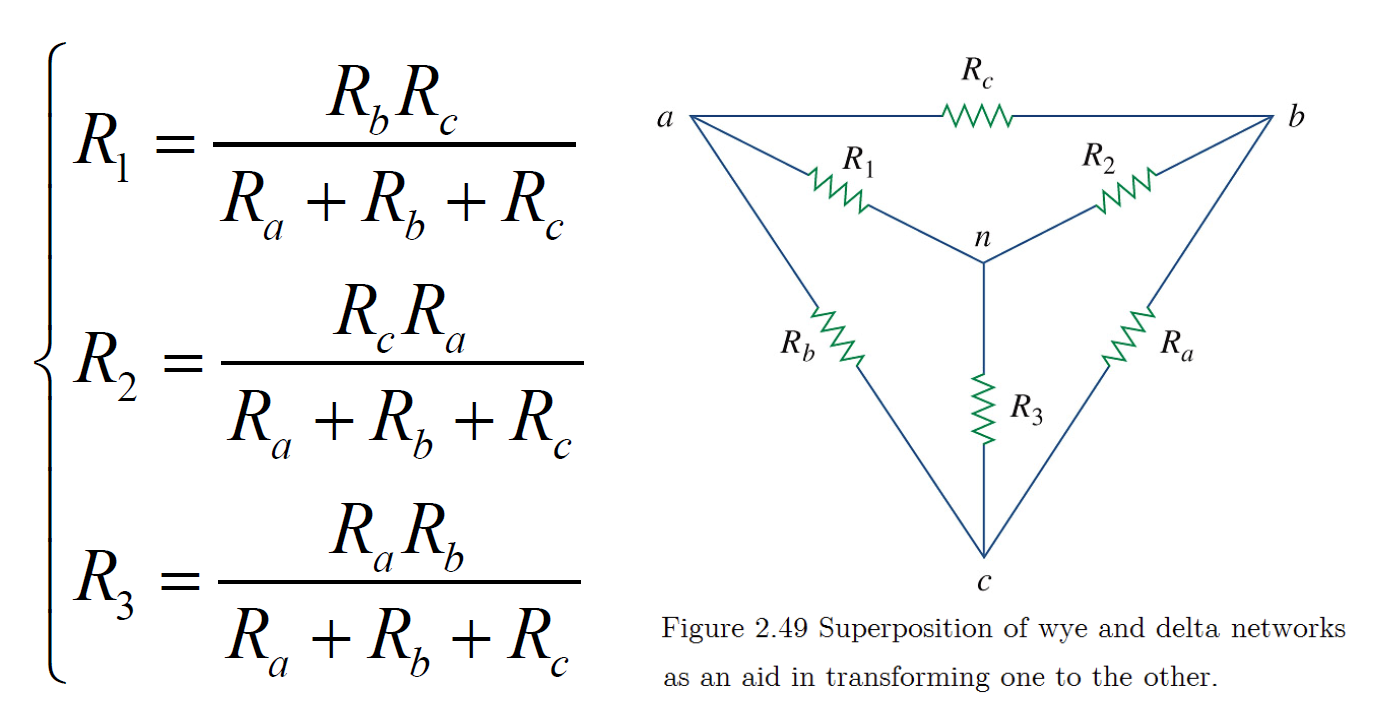
\includegraphics[width=0.7\textwidth]{34.png}
\caption{\Delta-Y}
\end{figure}

Intuition: parallel $\rightarrow$ series, resistance for each element decreases.

\end{frame}

%%%%%%%%%%%%%%%%%%%%%%%%%%%%%
\begin{frame}
\frametitle{Wye-Delta Transformation}
\begin{figure}[H]
\centering
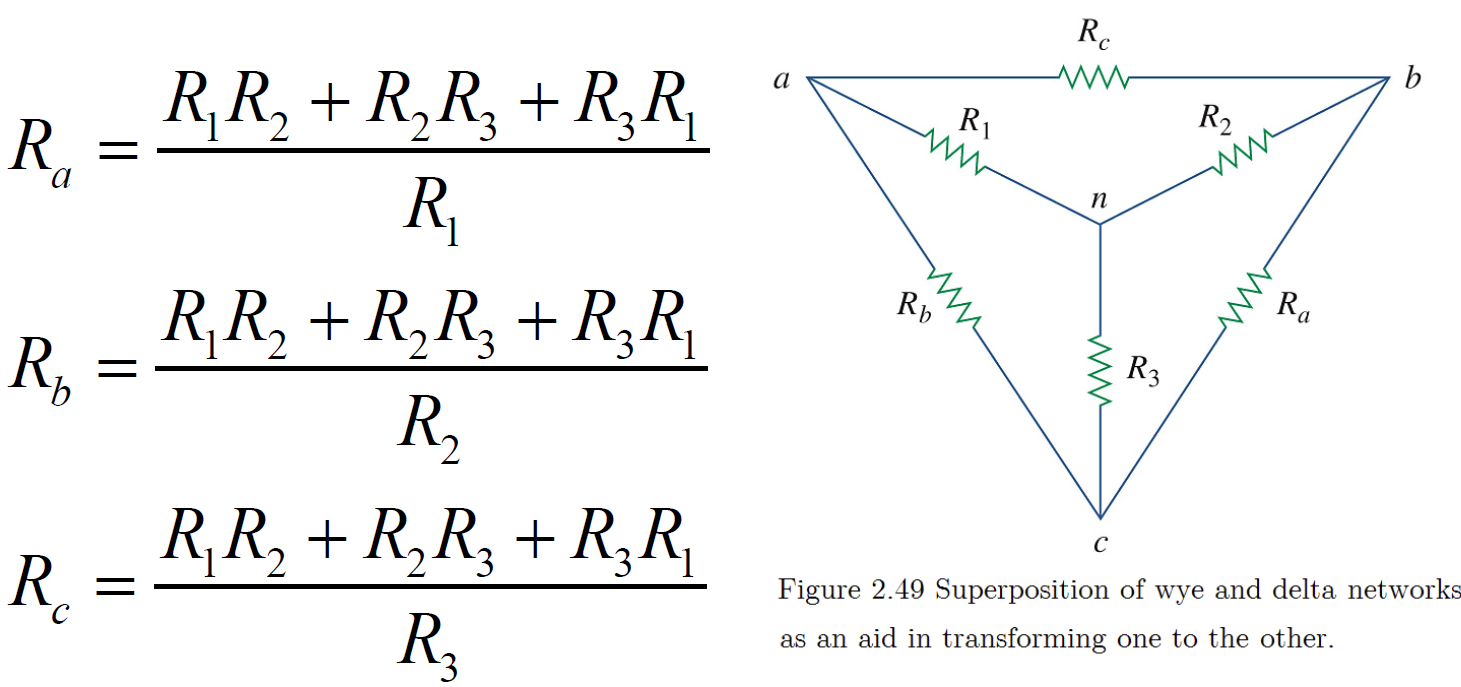
\includegraphics[width=0.7\textwidth]{35.png}
\caption{Y-\Delta}
\end{figure}

Intuition: series $\rightarrow$ parallel, resistance for each element increases.

\end{frame}

\begin{frame}{Exercise}
Calculate the equivalent resistance $R_{ab}$ in the circuit
\begin{figure}
\centering
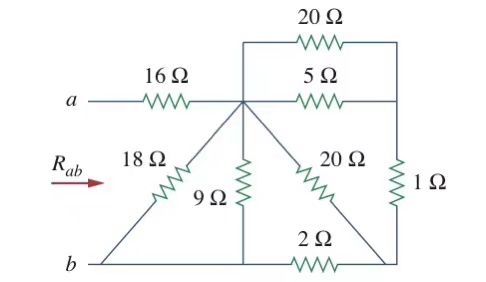
\includegraphics[width=3in]{32.jpg}
\end{figure}
\end{frame}

\begin{frame}{Exercise}
Calculate the equivalent resistance $R_{ab}$ in the circuit
\begin{figure}
\centering
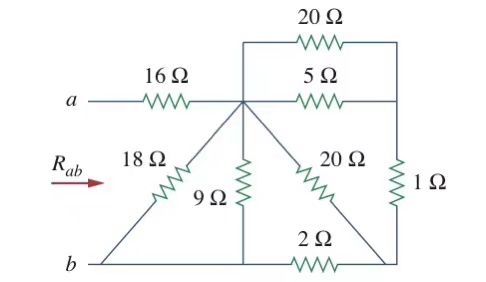
\includegraphics[width=3in]{32.jpg}
\end{figure}

\textbf{Answer:} 19$\Omega$
\end{frame}
\begin{frame}{Exercise}
\begin{figure}
\centering
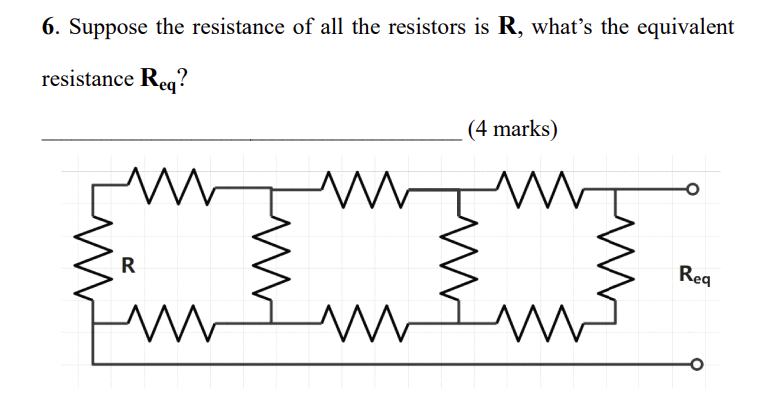
\includegraphics[width=0.8\textwidth]{Ex2.png}
\end{figure}
\end{frame}

\begin{frame}{Exercise}
\begin{figure}
\centering
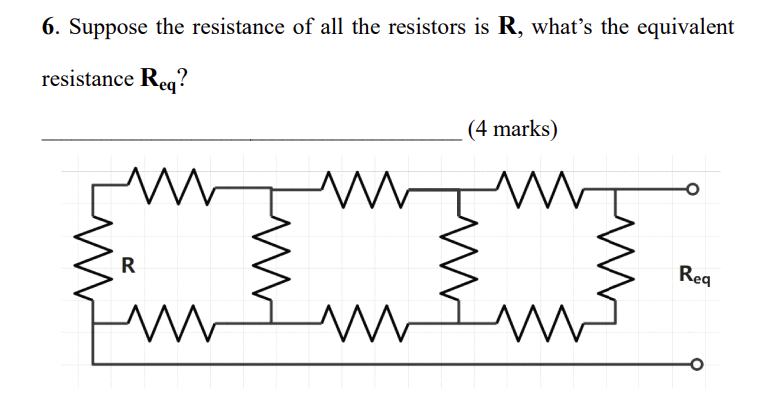
\includegraphics[width=0.7\textwidth]{Ex2.png}
\end{figure}
\centerline{\textbf{Answer:} $0.5+\dfrac{0.5+1+0.25}{2}+0.5=\dfrac{15}{8}R$}
\end{frame}


%-----------------------------------------------------
\section{Methods of Analysis}
\begin{frame}
\frametitle{Methods of Analysis}
Nodal Analysis:
\begin{enumerate}
    \item Select a reference node (ground)
    \item Apply KCL
    \item Solve the equations
\end{enumerate}
Mesh Analysis:
\begin{enumerate}
    \item Mark the current of all the meshes
    \item Apply KVL
    \item Solve the equations
\end{enumerate}

\end{frame}
%------------------------------------------------
\begin{frame}
\frametitle{Analysis by Inspection}
\begin{figure}[H]
        \centering
        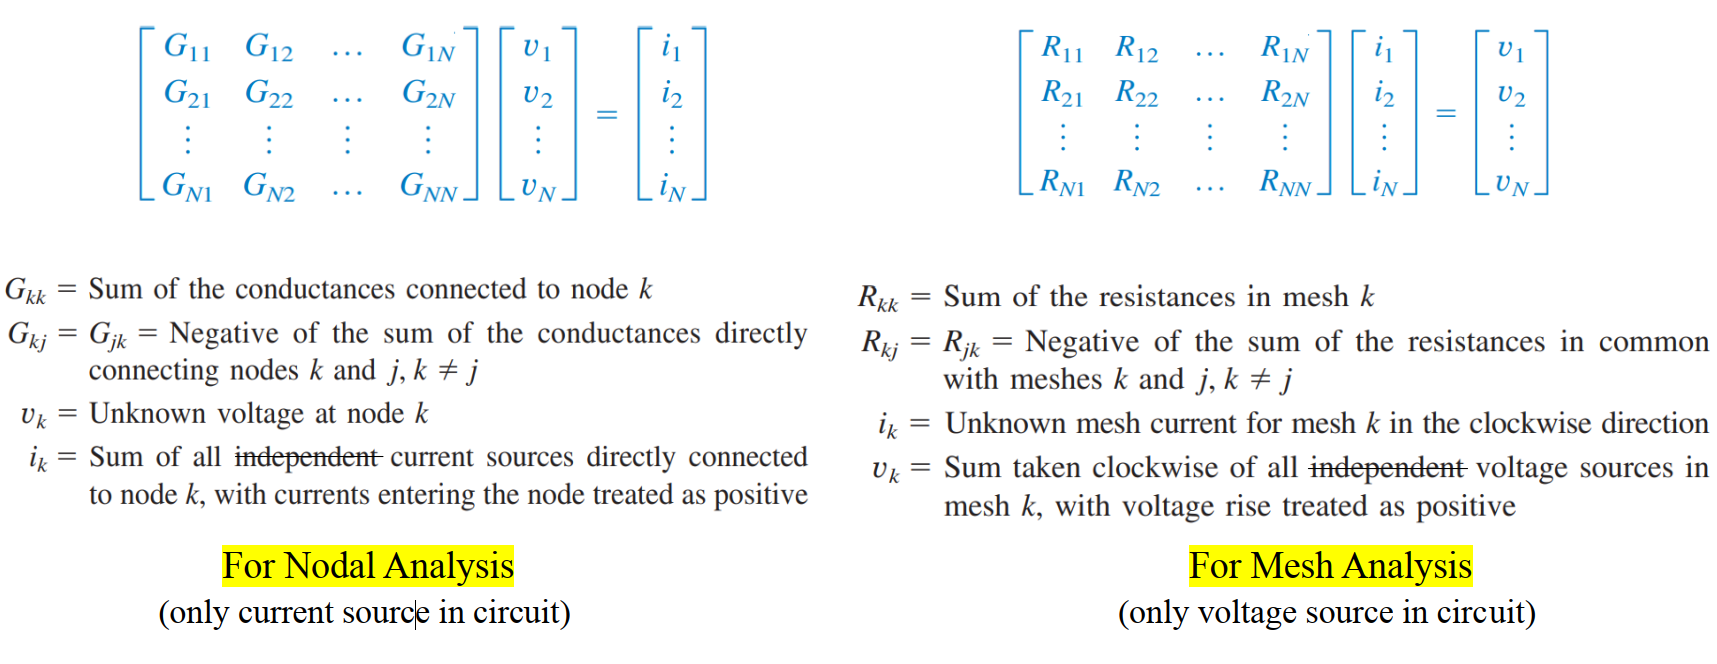
\includegraphics[width=1\textwidth]{ycy/analysis.png}
    \end{figure}
\end{frame}
%------------------------------------------------
\begin{frame}
\frametitle{Supernode \& Supermesh}
\begin{figure}[H]
        \centering
        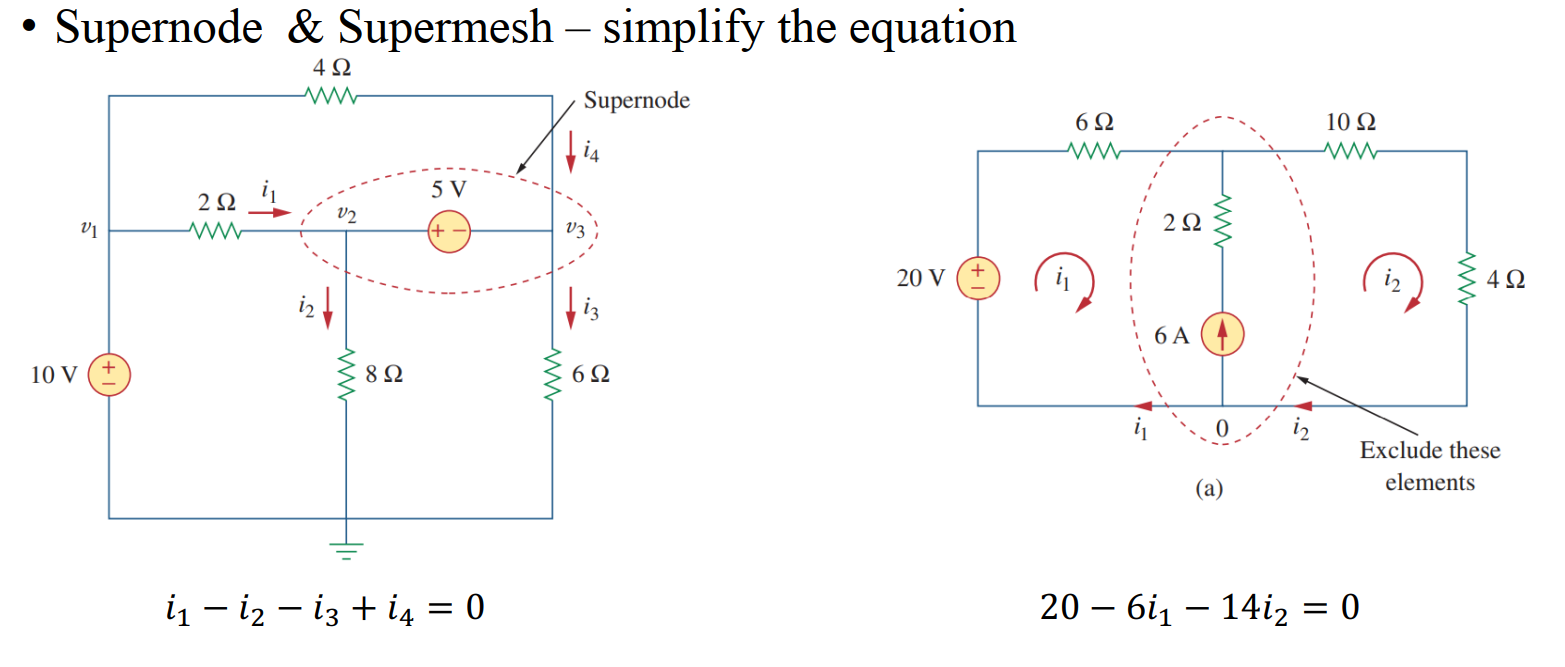
\includegraphics[width=1\textwidth]{ycy/super.png}
    \end{figure}
\end{frame}
%------------------------------------------------
\begin{frame}
\frametitle{Exercise}
\begin{figure}[H]
        \centering
        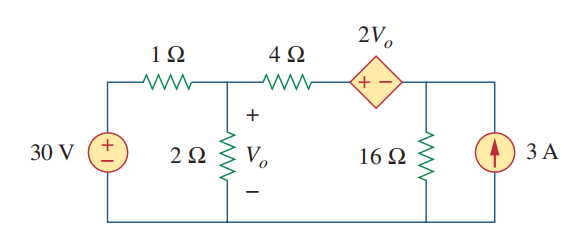
\includegraphics[width=1\textwidth]{ycy/exer.png}
    \end{figure}
\end{frame}

\begin{frame}
\frametitle{Exercise}
\begin{figure}[H]
        \centering
        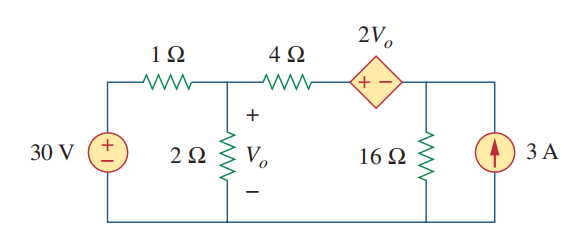
\includegraphics[width=1\textwidth]{ycy/exer.png}
    \end{figure}
\centerline{\textbf{Answer:} $\frac{648}{29} V \approx 22.34V$ }
\end{frame}



%%%%%%%%%%%%%%%%%%%%%%%%%%%%%%%%%%%%%%%%%%%%%%%%%%%



\begin{frame}
\frametitle{References}
\begin{enumerate}
\item 2022Fall VE215 slides
\item 2022Fall RC1, Zhiyu Zhou
\item 2022Summer RC1, Jiahui Wang
\end{enumerate}
\end{frame}


\begin{frame}
\Huge{\centerline{Thank you!}}
\end{frame}


\end{document}
